%!TEX program = xelatex
\documentclass{main}

\captionsetup{font=large}  % 使用 small 字体

\setmainfont{Times New Roman}
\setlength{\headheight}{13pt}
\usepackage{algpseudocode}
\usepackage{algorithm}
\usepackage{minted2}
\usepackage{minted}
\usepackage{tocloft}

% 设置目录标题格式
\renewcommand{\cfttoctitlefont}{\hfill\zihao{-2}\heiti}
\renewcommand{\cftaftertoctitle}{\hfill}

% 设置目录中的字体和行距
\renewcommand{\cftpartfont}{\zihao{4}\heiti}
\renewcommand{\cftsecfont}{\zihao{-4}\songti}
\renewcommand{\cftsubsecfont}{\zihao{-4}\songti}
\renewcommand{\cftsubsubsecfont}{\zihao{-4}\songti}

% 设置页码数字的字体
\renewcommand{\cftpartpagefont}{\zihao{4}\heiti}
\renewcommand{\cftsecpagefont}{\zihao{-4}\songti}
\renewcommand{\cftsubsecpagefont}{\zihao{-4}\songti}
\renewcommand{\cftsubsubsecpagefont}{\zihao{-4}\songti}

% 设置缩进
\setlength{\cftpartindent}{0em}
\setlength{\cftsecindent}{2em}
\setlength{\cftsubsecindent}{4em}
\setlength{\cftsubsubsecindent}{4em}

% 设置章节号后的格式
\renewcommand{\cftpartaftersnum}{}
\renewcommand{\cftsecaftersnum}{\hspace{0.5em}}
\renewcommand{\cftsubsecaftersnum}{\hspace{0.5em}}
\renewcommand{\cftsubsubsecaftersnum}{\hspace{0.5em}}

% 设置各级标题间距
\setlength{\cftbeforesecskip}{0.5ex}
\setlength{\cftbeforesubsecskip}{0.3ex}
\setlength{\cftbeforesubsubsecskip}{0.2ex}
% 设置目录行距为1.25倍
\renewcommand{\baselinestretch}{1.25}
% 定义目录标题
\renewcommand{\contentsname}{\centerline{目 \quad 录}}

% 调整目录层级显示
\setcounter{tocdepth}{3}
\setcounter{secnumdepth}{3}

\begin{document}

\thispagestyle{empty}

\begin{figure}[ht]
  \centering
  
\includegraphics[width=\linewidth]{./cover/scnu.jpg}
\end{figure}

\begin{center}
\zihao{0}
\textbf{本科毕业设计}
\end{center}

\begin{center}
\zihao{1}
\ \\\ \\\ \\
\end{center}

\begin{spacing}{1.8}

\begin{table}[ht]
  \zihao{-3}
  \setlength\extrarowheight{10pt}
  \centering
  \begin{tabular}{lc}
    \multicolumn{1}{c}{\textbf{题\hspace{\fill}目:\ }} & \textbf{一种多阶段密钥交换协议的设计与实现} \\ \cline{2-2} 
    % \multicolumn{1}{c}{\textbf{}} & \textbf{} \\ \cline{2-2} 
    \multicolumn{1}{c}{\textbf{指导老师:\ }} & \textbf{王立斌}             \\ \cline{2-2} 
    \multicolumn{1}{c}{\textbf{学生姓名:\ }}  & \textbf{史豪}             \\ \cline{2-2} 
    \multicolumn{1}{c}{\textbf{学\hspace{\fill}号:}}  & \textbf{20212131041}     \\ \cline{2-2} 
    \multicolumn{1}{c}{\textbf{学\hspace{\fill}院:}}  & \textbf{计算机学院}     \\ \cline{2-2} 
    \multicolumn{1}{c}{\textbf{专\hspace{\fill}业:}}  & \textbf{计算机科学与技术}            \\ \cline{2-2} 
    \multicolumn{1}{c}{\textbf{班\hspace{\fill}级:\ }}  & \textbf{1班}            \\ \cline{2-2} 
  \end{tabular}
\end{table}

\end{spacing}
\afterpage{\blankpage}
\newpage % 封面
\begin{spacing}{1.5}
\setboolean{@twoside}{true}
\zihao{-4}
\setcounter{page}{1}
\pagenumbering{arabic}

% \addcontentsline{toc}{section}{目录}
\tableofcontents
\newpage
\section{课题背景及设计目标}

\subsection{课题背景}

随着网络应用的日益普及,安全通信成为现代网络基础设施的核心需求。密钥交换协议允许通信双方在不安全的网络环境中建立共享密钥,为后续的安全通信提供基础。传统密钥交换协议如Diffie-Hellman和RSA在经典计算环境下已被广泛采用,但随着量子计算技术的迅速发展,这些依赖于离散对数和大整数分解难题的密码学原语面临着严峻挑战。

美国国家标准与技术研究院(NIST)于2016年启动后量子密码标准化竞赛,并于2022年公布了首批后量子密码标准算法。其中,基于格的密码学因其安全性依赖于格问题的计算困难性,被认为能够抵抗量子计算攻击,成为后量子密码学研究的重点方向。

传统的密钥交换协议通常将密钥建立与后续安全通信视为分离的阶段。然而,现代网络协议如TLS 1.3、QUIC和Signal等为了提高效率,往往将这些阶段交织在一起,通过多轮协商导出最终密钥。多阶段密钥交换(Multi-stage Key Exchange, MSKE)模型正是为了描述这种复杂交互过程而提出的。MSKE协议将整个交互划分为多个独立阶段,不同阶段可以采用不同的密钥协商与派生方式,生成的阶段密钥可用于不同目的,如消息加密、认证或完整性保护等。

基于密钥封装机制(Key Encapsulation Mechanism, KEM)的密钥交换协议在后量子安全性、高效性和设计简洁性方面具有显著优势。与传统公钥加密(PKE)相比,KEM更适合与混合加密方案结合使用,为现代密码协议提供标准化框架。NIST后量子密码标准中的多个算法都采用KEM设计范式,如基于模格的密钥封装(ML-KEM,前身为Kyber)。

为应对这一技术演进趋势,本文实现了一种紧致安全多阶段密钥交换协议(TIghtly secure Multi-stage Key Exchange,TIMKE),基于后量子安全的KEM构建,特别关注紧致安全性、后量子安全性和实际应用需求。

\subsection{设计目标}

本设计的主要目标是实现一个基于KEM的两阶段紧致安全多阶段密钥交换协议,满足现代网络应用对安全性、效率和灵活性的要求。具体设计目标如下:

\subsubsection{安全目标}

\begin{itemize}
    \item \textbf{后量子安全性}:协议采用基于格的密码学原语,其安全性依赖于在量子计算模型下仍被认为困难的格问题,确保在量子计算时代保持安全性。
    
    \item \textbf{紧致安全性}:协议安全性证明中的归约损失不随会话数量线性增长,确保在大规模部署环境中维持高安全边际。
    
    \item \textbf{多阶段安全性}:支持两阶段密钥派生,第二阶段提供弱前向安全性(即使服务器长期密钥泄露,只要对第二阶段仅采取被动攻击,主会话密钥仍能保持安全)。
    
    \item \textbf{单边认证安全性}:仅对服务器进行身份认证,客户端可匿名参与,简化协议设计并满足普通Web访问等场景的安全需求。
\end{itemize}

\subsubsection{功能目标}

\begin{itemize}
    \item \textbf{双阶段密钥派生}:实现两阶段密钥派生机制,第一阶段基于OW-ChCCA安全的KEM,第二阶段基于OW-PCA安全的KEM,满足不同安全需求。
    
    \item \textbf{0-RTT数据传输}:支持零往返时间数据传输,允许客户端在首个消息中直接发送加密应用数据,显著减少连接建立延迟。
    
    \item \textbf{通用构造与灵活配置}:支持集成不同的后量子安全KEM算法,如ML-KEM、自定义OW-ChCCA KEM等,提供参数优化选项适应不同使用场景。
    
    \item \textbf{实用性能平衡}:在保证安全性的前提下,优化计算效率和通信开销,使协议在普通计算设备上可行运行。
\end{itemize}

\subsubsection{技术要求}

\begin{itemize}
    \item \textbf{模块化设计}:采用严格的模块化架构,使各组件可独立更新和维护,提高代码可读性和可维护性。
    
    \item \textbf{接口标准化}:设计统一的KEM接口,支持不同KEM算法的无缝集成,确保协议在不同环境中的可适配性。
    
    \item \textbf{全面测试验证}:构建完整的测试套件,包括单元测试、集成测试和性能测试,验证协议在各种条件下的正确性和安全性。
    
    \item \textbf{开源可用}:提供可重用的开源实现,支持社区审查和改进,促进后量子安全通信技术的推广。
\end{itemize}

通过实现这些设计目标,本项目旨在为后量子安全通信提供一个理论上严格、实践中可行的解决方案,填补目前在多阶段密钥交换协议实际实现方面的空白。
\section{系统设计}

\subsection{系统架构设计}

TIMKE协议实现采用分层架构和模块化设计,将各功能组件高度解耦,提高系统的可维护性、可测试性和可扩展性。整体架构分为五个核心层次,如图\ref{fig:system-architecture}所示:

\begin{figure}[H]
  \centering
  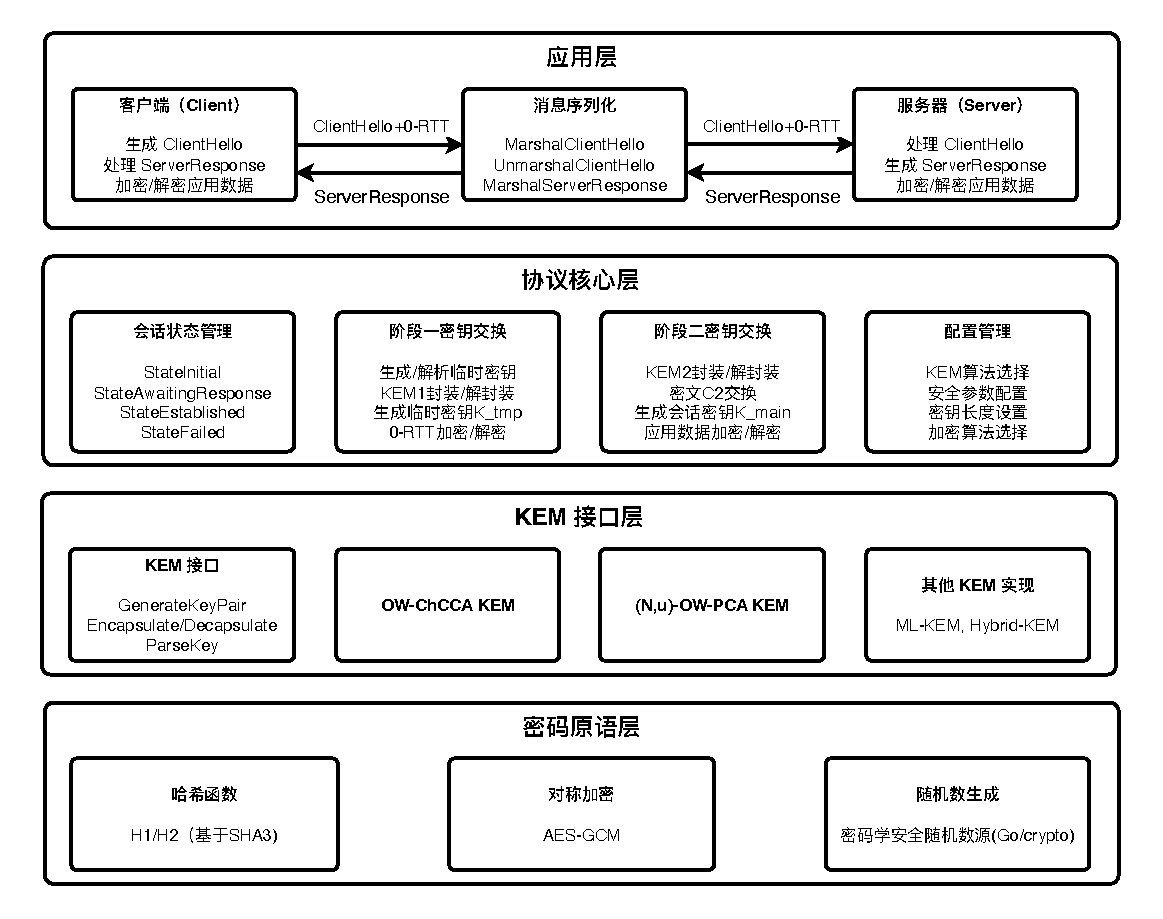
\includegraphics[width=0.9\textwidth]{figures/implementation.drawio.pdf}
  \caption{TIMKE协议实现架构}
  \label{fig:system-architecture}
\end{figure}

\subsubsection{应用层}
应用层提供用户界面和演示功能,封装了Client和Server实体,支持完整的协议交互和0-RTT数据传输。该层主要由以下组件构成:

\begin{itemize}
    \item \textbf{客户端程序}:负责启动密钥交换流程、发送0-RTT数据并与服务器进行加密通信,支持交互式和批处理两种运行模式。
    
    \item \textbf{服务器程序}:负责接收连接请求、处理密钥协商消息并响应客户端,支持多客户端并发连接。
    
    \item \textbf{演示脚本}:提供用户友好的命令行界面,自动化协议测试流程,让用户无需了解底层实现细节即可体验协议功能。
\end{itemize}

\subsubsection{序列化层}
序列化层负责协议消息的编码与解码,确保跨平台通信的一致性和正确性。主要组件包括:

\begin{itemize}
    \item \textbf{消息定义}:定义ClientHello和ServerResponse两种主要消息结构,包含必要的协议字段和可选扩展。
    
    \item \textbf{编码/解码器}:实现二进制格式的消息序列化和反序列化,使用长度前缀和稠密编码优化通信效率。
    
    \item \textbf{协议协商支持}:通过消息字段支持KEM类型协商,允许客户端和服务器动态选择兼容的加密算法。
\end{itemize}

\subsubsection{协议核心层}
协议核心层实现TIMKE协议的状态管理、会话处理和密钥协商逻辑,是整个系统的核心。主要组件包括:

\begin{itemize}
    \item \textbf{会话状态管理}:定义并管理协议的四种核心状态(Initial、AwaitingServerResponse、Established、Failed),确保协议操作顺序和安全性。
    
    \item \textbf{阶段一密钥交换}:实现临时会话密钥的协商和0-RTT数据的加密/解密,支持初始连接的低延迟通信。
    
    \item \textbf{阶段二密钥交换}:实现具有弱前向安全性的主会话密钥协商,用于后续通信的高强度安全保障。
    
    \item \textbf{配置管理}:处理KEM算法选择、安全参数配置等协议设置,支持灵活的部署选项。
\end{itemize}

\subsubsection{KEM接口层}
KEM接口层定义统一的密钥封装机制接口,实现算法无关的操作抽象,允许协议灵活嵌入不同的KEM实现。主要组件包括:

\begin{itemize}
    \item \textbf{KEM接口定义}:规范化的KEM操作集,包括密钥生成、封装、解封装等核心功能。
    
    \item \textbf{OW-ChCCA KEM实现}:基于格密码学的单向可检测选择密文安全KEM实现,是协议安全证明的直接对应。
    
    \item \textbf{ML-KEM集成}:集成NIST标准的后量子KEM算法,提供高效的实用替代方案。
    
    \item \textbf{KEM注册表}:通过工厂模式和注册表模式管理不同KEM算法,支持运行时动态选择。
\end{itemize}

\subsubsection{密码原语层}
密码原语层提供哈希函数、对称加密等基础密码学功能,为协议的密钥派生和数据加密提供支持。主要组件包括:

\begin{itemize}
    \item \textbf{哈希函数}:基于SHA3实现的H1和H2密钥派生函数,支持临时会话密钥和主会话密钥的安全派生。
    
    \item \textbf{对称加密}:基于AES-GCM的加密方案,为0-RTT数据和后续通信提供机密性和完整性保护。
    
    \item \textbf{随机数生成}:密码学安全的随机数源,用于密钥生成和防重放保护。
\end{itemize}

这种分层设计严格遵循关注点分离原则,使各组件能够独立演化和测试。同时,通过定义清晰的接口,系统支持在不修改协议核心逻辑的情况下替换或更新各层组件,为协议的长期维护和演进奠定了坚实基础。

\subsection{功能模块设计}

\subsubsection{协议参与方与工作流程}

TIMKE协议涉及两个参与方:客户端(C)和服务器(S),它们通过两个阶段的交互完成密钥协商。整体工作流程如图\ref{fig:protocol-flow}所示:

\begin{figure}[H]
  \centering
  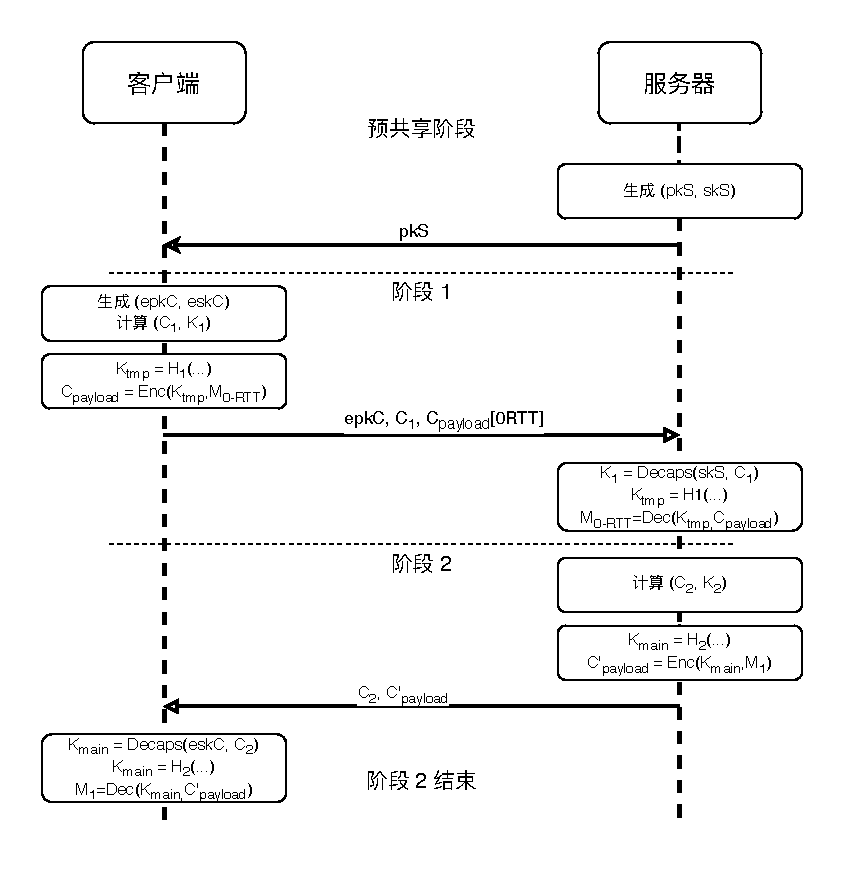
\includegraphics[width=0.8\textwidth]{figures/protocol.drawio.pdf}
  \caption{TIMKE协议工作流程}
  \label{fig:protocol-flow}
\end{figure}

\paragraph{预共享阶段}
在正式协议交互前,服务器生成长期密钥对$(pk_S, sk_S)$,并通过可信渠道将公钥$pk_S$分发给客户端。这一阶段类似于TLS中的证书分发过程。

\paragraph{第一阶段:临时密钥协商与0-RTT传输}
\begin{enumerate}
    \item 客户端生成临时密钥对$(epk_C, esk_C)$并使用服务器公钥封装共享密钥$(C_1, K_1)$
    \item 客户端派生临时会话密钥$K_{tmp} = H_1(pk_S, C_1, K_1)$
    \item 客户端使用$K_{tmp}$加密0-RTT数据$C_{payload}$并发送$(epk_C, C_1, C_{payload})$
    \item 服务器使用私钥解封装得到$K_1$,派生相同的$K_{tmp}$并解密0-RTT数据
\end{enumerate}

\paragraph{第二阶段:主会话密钥建立}
\begin{enumerate}
    \item 服务器使用客户端临时公钥封装共享密钥$(C_2, K_2)$
    \item 服务器派生主会话密钥$K_{main} = H_2(pk_S, epk_C, C_1, C_2, K_1, K_2)$
    \item 服务器加密应用数据并发送$(C_2, C'_{payload})$
    \item 客户端解封装得到$K_2$,派生相同的$K_{main}$并解密服务器数据
\end{enumerate}

\subsubsection{密钥封装机制实现}

作为TIMKE协议的核心组件,系统实现了两类KEM算法:

\paragraph{OW-ChCCA KEM}
单向可检测选择密文安全KEM是TIMKE协议安全证明的基础,基于格密码学构建,具体实现包括:

\begin{itemize}
    \item \textbf{密钥结构}:公钥包含矩阵$\mathbf{A}$、$\mathbf{u}_0$、$\mathbf{u}_1$;私钥包含矩阵$\mathbf{Z}_b$和标志位$b$
    \item \textbf{密钥生成}:从均匀分布随机采样$\mathbf{A}$,从高斯分布采样$\mathbf{Z}_b$,计算$\mathbf{A}\mathbf{Z}_b$
    \item \textbf{封装/解封装}:基于学习带误差(LWE)问题构建的安全机制
    \item \textbf{参数优化}:针对实际应用环境,调整理论参数以平衡安全性和性能
\end{itemize}

\paragraph{ML-KEM集成}
为提供更高效的实现方案,系统集成了NIST标准的ML-KEM算法:

\begin{itemize}
    \item \textbf{支持级别}:ML-KEM-512(AES-128等效安全级别)、ML-KEM-768(AES-192等效)、ML-KEM-1024(AES-256等效)
    \item \textbf{接口适配}:通过统一KEM接口封装ML-KEM操作,实现无缝集成
    \item \textbf{性能优化}:利用ML-KEM的高效实现提升整体协议性能
\end{itemize}

\subsubsection{消息格式与处理}

系统定义了两种主要消息类型,用于客户端和服务器之间的交互:

\paragraph{ClientHello消息}
客户端发送的第一个消息,包含以下字段:
\begin{itemize}
    \item \textbf{EphemeralPublicKey}:客户端临时公钥$epk_C$
    \item \textbf{Ciphertext1}:使用服务器公钥封装的密文$C_1$
    \item \textbf{EncryptedPayload}:使用临时会话密钥加密的0-RTT数据(可选)
    \item \textbf{KEM1Type/KEM2Type}:用于指示使用的KEM类型(用于协商)
\end{itemize}

\paragraph{ServerResponse消息}
服务器对ClientHello的响应,包含以下字段:
\begin{itemize}
    \item \textbf{Ciphertext2}:使用客户端临时公钥封装的密文$C_2$
    \item \textbf{EncryptedPayload}:使用主会话密钥加密的应用数据(可选)
\end{itemize}

消息序列化采用长度前缀编码方式,确保跨平台兼容性和传输效率。

\subsubsection{会话状态管理}

系统采用状态机模式管理协议状态,定义了四种核心状态:

\begin{itemize}
    \item \textbf{StateInitial}:初始状态,表示会话尚未开始
    \item \textbf{StateAwaitingServerResponse}:客户端已发送请求,等待服务器响应
    \item \textbf{StateEstablished}:会话成功建立,可以安全通信
    \item \textbf{StateFailed}:会话建立失败,需要重新协商
\end{itemize}

状态转换逻辑确保协议严格按照预定流程执行,防止状态错误导致的安全问题。每个状态转换都包含完整的错误处理逻辑,保证在异常情况下能够正确回退或终止会话。

\subsubsection{密钥派生机制}

协议中的密钥派生是安全性的关键环节,实现了两个专用的密钥派生函数:

\begin{itemize}
    \item \textbf{H1函数}:派生临时会话密钥,$K_{tmp} = H_1(pk_S, C_1, K_1)$
    \item \textbf{H2函数}:派生主会话密钥,$K_{main} = H_2(pk_S, epk_C, C_1, C_2, K_1, K_2)$
\end{itemize}

这些函数基于SHA3-512哈希函数实现,采用域分隔技术增强安全性,确保不同上下文的哈希值不会发生冲突。密钥派生过程包括完整的输入验证,确保不会处理无效数据。

\subsubsection{扩展性与配置机制}

系统设计重视扩展性与灵活配置,提供多层次的配置接口:

\begin{itemize}
    \item \textbf{KEM算法配置}:支持多种KEM组合,如ML-KEM-768/1024或OWChCCA/ML-KEM混合
    \item \textbf{安全参数选择}:允许根据应用需求选择不同安全级别
    \item \textbf{会话选项配置}:通过SessionOptions接口灵活配置会话参数
\end{itemize}

所有核心组件均通过接口定义,支持替换具体实现。系统使用注册机制管理KEM算法,便于添加新的算法实现。这种设计确保系统能够随着密码学研究进展和安全需求变化而演进,延长协议实现的生命周期。
\section{开发工具与运行环境}

\subsection{开发工具}

本项目采用现代软件工程方法进行开发,使用了以下主要开发工具:

\begin{itemize}
    \item \textbf{编程语言}:主要使用Go语言(版本1.23.4)进行开发,该语言具有以下优势:
    \begin{itemize}
        \item 强大的并发处理能力,适合高性能密码学应用
        \item 完善的标准库,包括丰富的密码学原语支持
        \item 强类型系统和内存安全特性,减少常见安全漏洞
        \item 跨平台兼容性,支持多种操作系统和硬件架构
    \end{itemize}
    
    \item \textbf{开发环境}:
    \begin{itemize}
        \item Visual Studio Code:主要代码编辑器,配置了Go语言插件集成
        \item GoLand:JetBrains公司的Go专用IDE,提供高级调试和代码分析功能
        \item Git:版本控制系统,用于代码管理和协作
        \item GitHub:代码托管平台,用于项目公开和分享
    \end{itemize}
    
    \item \textbf{测试工具}:
    \begin{itemize}
        \item Go内置测试框架:用于单元测试和集成测试
        \item Go Benchmark:用于性能测试和比较
        \item Bash脚本:用于自动化测试和演示
    \end{itemize}
    
    \item \textbf{文档工具}:
    \begin{itemize}
        \item Markdown:编写项目文档和说明
        \item LaTeX:编写学术论文和技术报告
        \item Draw.io:创建系统架构和流程图
    \end{itemize}
\end{itemize}

\subsection{运行环境}

TIMKE协议实现设计为可在多种环境下运行,以下是推荐的运行环境配置:

\subsubsection{硬件要求}

\begin{itemize}
    \item \textbf{CPU}:现代多核处理器(推荐4核心或以上)
    \item \textbf{内存}:
    \begin{itemize}
        \item 基础运行:最低4GB RAM
        \item OW-ChCCA实现:推荐16GB以上RAM
        \item ML-KEM实现:4GB RAM即可满足需求
    \end{itemize}
    \item \textbf{存储}:至少200MB可用空间(源代码、编译产物和演示数据)
    \item \textbf{网络}:支持TCP/IP网络连接(用于客户端-服务器通信)
\end{itemize}

\subsubsection{软件环境}

\begin{itemize}
    \item \textbf{操作系统}:
    \begin{itemize}
        \item Linux(Ubuntu 20.04+,CentOS 8+等)
        \item macOS(10.15+)
        \item Windows 10/11(使用Windows Subsystem for Linux或原生Go环境)
    \end{itemize}
    
    \item \textbf{运行时依赖}:
    \begin{itemize}
        \item Go语言运行时(1.18+,推荐1.23+)
        \item Bash 4.0+(用于演示脚本)
    \end{itemize}
    
    \item \textbf{库依赖}:
    \begin{itemize}
        \item Cloudflare的CIRCL库:提供ML-KEM等后量子密码学实现
        \item Tuneinsight的Lattigo库:提供格密码学相关功能
        \item 标准Go库中的crypto包:提供基础密码学功能
    \end{itemize}
\end{itemize}

值得注意的是,不同KEM算法配置对系统资源的要求差异较大。使用ML-KEM配置时,系统资源需求较低,适合包括移动设备在内的各类环境;而使用自实现的OW-ChCCA KEM时,特别是高安全级别配置,需要更多内存和处理能力。

\subsubsection{开发环境配置}

本项目的开发和测试主要在以下环境中进行:

\begin{itemize}
    \item \textbf{操作系统}:macOS Sequoia 15
    \item \textbf{处理器}:Apple M1 Pro(8核,6性能/2能效)
    \item \textbf{内存}:16GB RAM
    \item \textbf{Go版本}:1.23.4
    \item \textbf{编辑器}:Visual Studio Code / GoLand
    \item \textbf{终端}:iTerm2 + Bash
\end{itemize}

\subsection{安装方法}

以下为TIMKE协议实现的安装步骤,适用于不同操作系统环境:

\subsubsection{前提条件}

确保系统已安装:
\begin{itemize}
    \item Go语言环境(1.18或更高版本)
    \item Git版本控制工具
    \item Bash shell(Linux/macOS自带,Windows需安装Git Bash或WSL)
\end{itemize}

\subsubsection{获取源代码}

通过Git克隆项目仓库:
\begin{minted}[breaklines]{bash}
# 克隆主项目仓库
git clone https://github.com/MingLLuo/TIMKE.git

# 克隆OW-ChCCA-KEM实现(如需使用)
git clone https://github.com/MingLLuo/OW-ChCCA-KEM.git
\end{minted}

\subsubsection{安装依赖}

项目使用Go模块管理依赖,自动下载所需库:

\begin{minted}[breaklines]{bash}
cd TIMKE
go mod download
\end{minted}

\subsubsection{编译项目}

编译客户端和服务器程序:

\begin{minted}[breaklines]{bash}
# 编译服务器
go build -o timke-server ./cmd/server

# 编译客户端
go build -o timke-client ./cmd/client

# 编译性能测试工具(可选)
go build -o kem-bench ./cmd/kemBench
go build -o protocol-bench ./cmd/protocolBench
\end{minted}

\subsubsection{配置环境变量(可选)}

为便于使用,可将程序路径添加到系统PATH:

\begin{minted}[breaklines]{bash}
# Linux/macOS
export PATH=$PATH:$(pwd)

# 永久添加(添加到~/.bashrc或~/.zshrc)
echo 'export PATH=$PATH:INSTALLATION_PATH' >> ~/.bashrc
\end{minted}

安装完成后,可通过项目提供的演示脚本体验完整功能:

\begin{minted}[breaklines]{bash}
# 运行演示脚本
cd TIMKE
./scripts/demo.bash
\end{minted}
通过以上步骤,您可以在本地环境中成功安装和运行TIMKE协议实现。
\section{功能演示}

\subsection{运行流程}

TIMKE协议实现提供了完整的演示系统,便于直观了解协议的工作原理和实际应用场景。本节将详细介绍系统的运行流程,从密钥生成到安全通信的完整过程。

\subsubsection{演示脚本概述}

项目提供了一个交互式演示脚本`demo.bash`,该脚本集成了所有核心功能并提供了用户友好的界面。通过该脚本,用户无需了解复杂的命令行参数,即可体验TIMKE协议的完整生命周期。

脚本启动后会显示如下菜单界面:

\begin{minted}[breaklines]{bash}
TIMKE Demo Options:
  1) Generate server keys
  2) Start server
  3) Run client with 0-RTT data
  4) Run client in interactive mode
  5) Show server log
  6) Stop server
  7) Exit

Using KEM1: ML-KEM-768, KEM2: ML-KEM-768, Port: 8443

Server is not running (stale PID file)

Enter your choice [1-7]: 
\end{minted}

用户可以按数字顺序操作,逐步体验协议各个阶段。

\subsubsection{密钥生成与服务器启动}

首先,需要生成服务器的长期密钥对,这是协议预共享阶段的核心步骤:

\begin{minted}[breaklines]{bash}
# 选择菜单选项1: Generate server keys
Enter your choice [1-7]: 1
\end{minted}

系统会输出密钥生成相关信息:

\begin{minted}[breaklines]{bash}

  Generating new ML-KEM-768 key pair...
  Key pair generated and saved to...
  Server public key (for client use): f64538fe52ab28f8cb9327ca30bc3cf0f97263d247b5374c633674322b35edbc...
  Long Term Key algorithm: ML-KEM-768
  
  Server keys generated:
    Private key: .temp/server-key.pem
    Public key: .temp/server-key.pem.pub
  
  Press Enter to continue...
\end{minted}

生成的服务器公钥将在后续客户端连接时使用,私钥则由服务器安全保存。接下来,启动服务器程序:

\begin{minted}[breaklines]{bash}
# 选择菜单选项2: Start server
Enter your choice [1-7]: 2
\end{minted}

系统会输出服务器启动的状态信息:

\begin{minted}[breaklines]{bash}
Starting TIMKE server on port 8443...
Server started with PID 12345
Server log available at: .temp/server.log
Tail of server log:
Available KEM algorithms:
  - ML-KEM-512
  - ML-KEM-768
  - ML-KEM-1024
  - OWChCCA-16
  - OWChCCA-32
  - OWChCCA-64

Loading private key from .temp/server-key.pem...
Private key loaded successfully
Server public key (for client use): f64538fe52ab28f8cb9327ca30bc3cf0f97263d247b5374c633674322b35edbc...
Long Term Key algorithm: ML-KEM-768

Server listening on port 8443...

Press Enter to continue...
\end{minted}

此时服务器已在指定端口监听,等待客户端连接。

\subsubsection{客户端连接与0-RTT数据传输}

服务器启动后,可以选择使用携带0-RTT数据的客户端进行连接:

\begin{minted}[breaklines]{bash}
# 选择菜单选项3: Run client with 0-RTT data
Enter your choice [1-7]: 3
\end{minted}

系统会输出客户端连接和0-RTT数据传输的过程:

\begin{minted}[breaklines]{bash}
Running TIMKE client with 0-RTT data...
Available KEM algorithms:
  - ML-KEM-512
  - ML-KEM-768
  - ML-KEM-1024
  - OWChCCA-16
  - OWChCCA-32
  - OWChCCA-64

Using server key: ML-KEM-768
Connecting to localhost:8443...
Connected to localhost:8443
Generating ClientHello...
Sent ClientHello (1438 bytes)
Sent 0-RTT data: "Hello from TIMKE client! This is 0-RTT data."
Waiting for server response...
Received server response (1424 bytes)
Session established! Protocol completed in 437µs
Server data: Hello from TIMKE server! This is stage-2 protected data.
TIMKE protocol completed successfully!

\end{minted}

从输出可以看到,客户端成功发送了携带0-RTT数据的ClientHello消息,并接收到服务器响应,建立了安全会话。整个过程耗时仅437微秒,展示了协议的高效性。

\subsubsection{交互式加密通信}

除了单次连接外,系统还支持交互式模式,允许用户在建立会话后发送多条加密消息:

\begin{minted}[breaklines]{bash}
# 选择菜单选项4: Run client in interactive mode
Enter your choice [1-7]: 4
\end{minted}

系统会进入交互式模式,用户可以输入消息并查看加密通信过程:

\begin{minted}[breaklines]{bash}
Running TIMKE client in interactive mode...
[连接和会话建立信息类似前面的输出]

Entering interactive mode. Type messages to send to server (type 'exit' to quit):
> Hello, this is a secure message!
Sent encrypted message (64 bytes)
Server: Server received: Hello, this is a secure message! (at 2025-03-20T15:42:36Z)

> Another encrypted message
Sent encrypted message (57 bytes)
Server: Server received: Another encrypted message (at 2025-03-20T15:42:45Z)

> exit
\end{minted}

交互式模式允许用户直观体验TIMKE协议的加密通信功能,所有消息都使用会话密钥加密传输,确保通信安全。

\subsubsection{日志查看与会话管理}

演示系统还提供了查看服务器日志和停止服务器的功能:

\begin{minted}[breaklines]{bash}
# 选择菜单选项5: Show server log
Enter your choice [1-7]: 5

# 选择菜单选项6: Stop server
Enter your choice [1-7]: 6
\end{minted}

通过这些功能,用户可以完整了解协议的运行状态和会话管理过程。

\subsection{运行效果}

本节展示TIMKE协议在不同配置下的运行效果,特别关注其实用性能和安全特性。

\subsubsection{协议运行效率}

TIMKE协议的运行效率与所选KEM算法密切相关。表\ref{tab:runtime-performance}展示了不同KEM组合下的协议执行时间:

\begin{table}[ht]
\centering
\caption{不同KEM组合的TIMKE协议运行效率}
\label{tab:runtime-performance}
\begin{tabular}{|l|r|r|r|}
\hline
\textbf{KEM组合} & \textbf{阶段1时间(ms)} & \textbf{阶段2时间(ms)} & \textbf{总时间(ms)} \\
\hline
ML-KEM-512 + ML-KEM-512    & 0.10  & 0.07  & 0.17   \\
\hline
ML-KEM-768 + ML-KEM-768    & 0.15  & 0.10  & 0.25   \\
\hline
ML-KEM-1024 + ML-KEM-1024  & 0.21  & 0.14  & 0.35   \\
\hline
OWChCCA-16 + ML-KEM-512    & 322.18  & 118.53  & 440.71   \\
\hline
\end{tabular}
\end{table}

从表中可以看出,使用ML-KEM配置时,协议可在毫秒级甚至亚毫秒级时间内完成,适合延迟敏感应用;而使用OWChCCA KEM配置时,由于其计算复杂度较高,运行时间显著增加,但仍在可接受范围内。

\subsubsection{0-RTT数据传输效果}

TIMKE协议支持0-RTT数据传输,允许客户端在首个往返中发送加密数据。图\ref{fig:0rtt-demo}展示了通过演示系统发送0-RTT数据的效果:

\begin{figure}[ht]
\centering
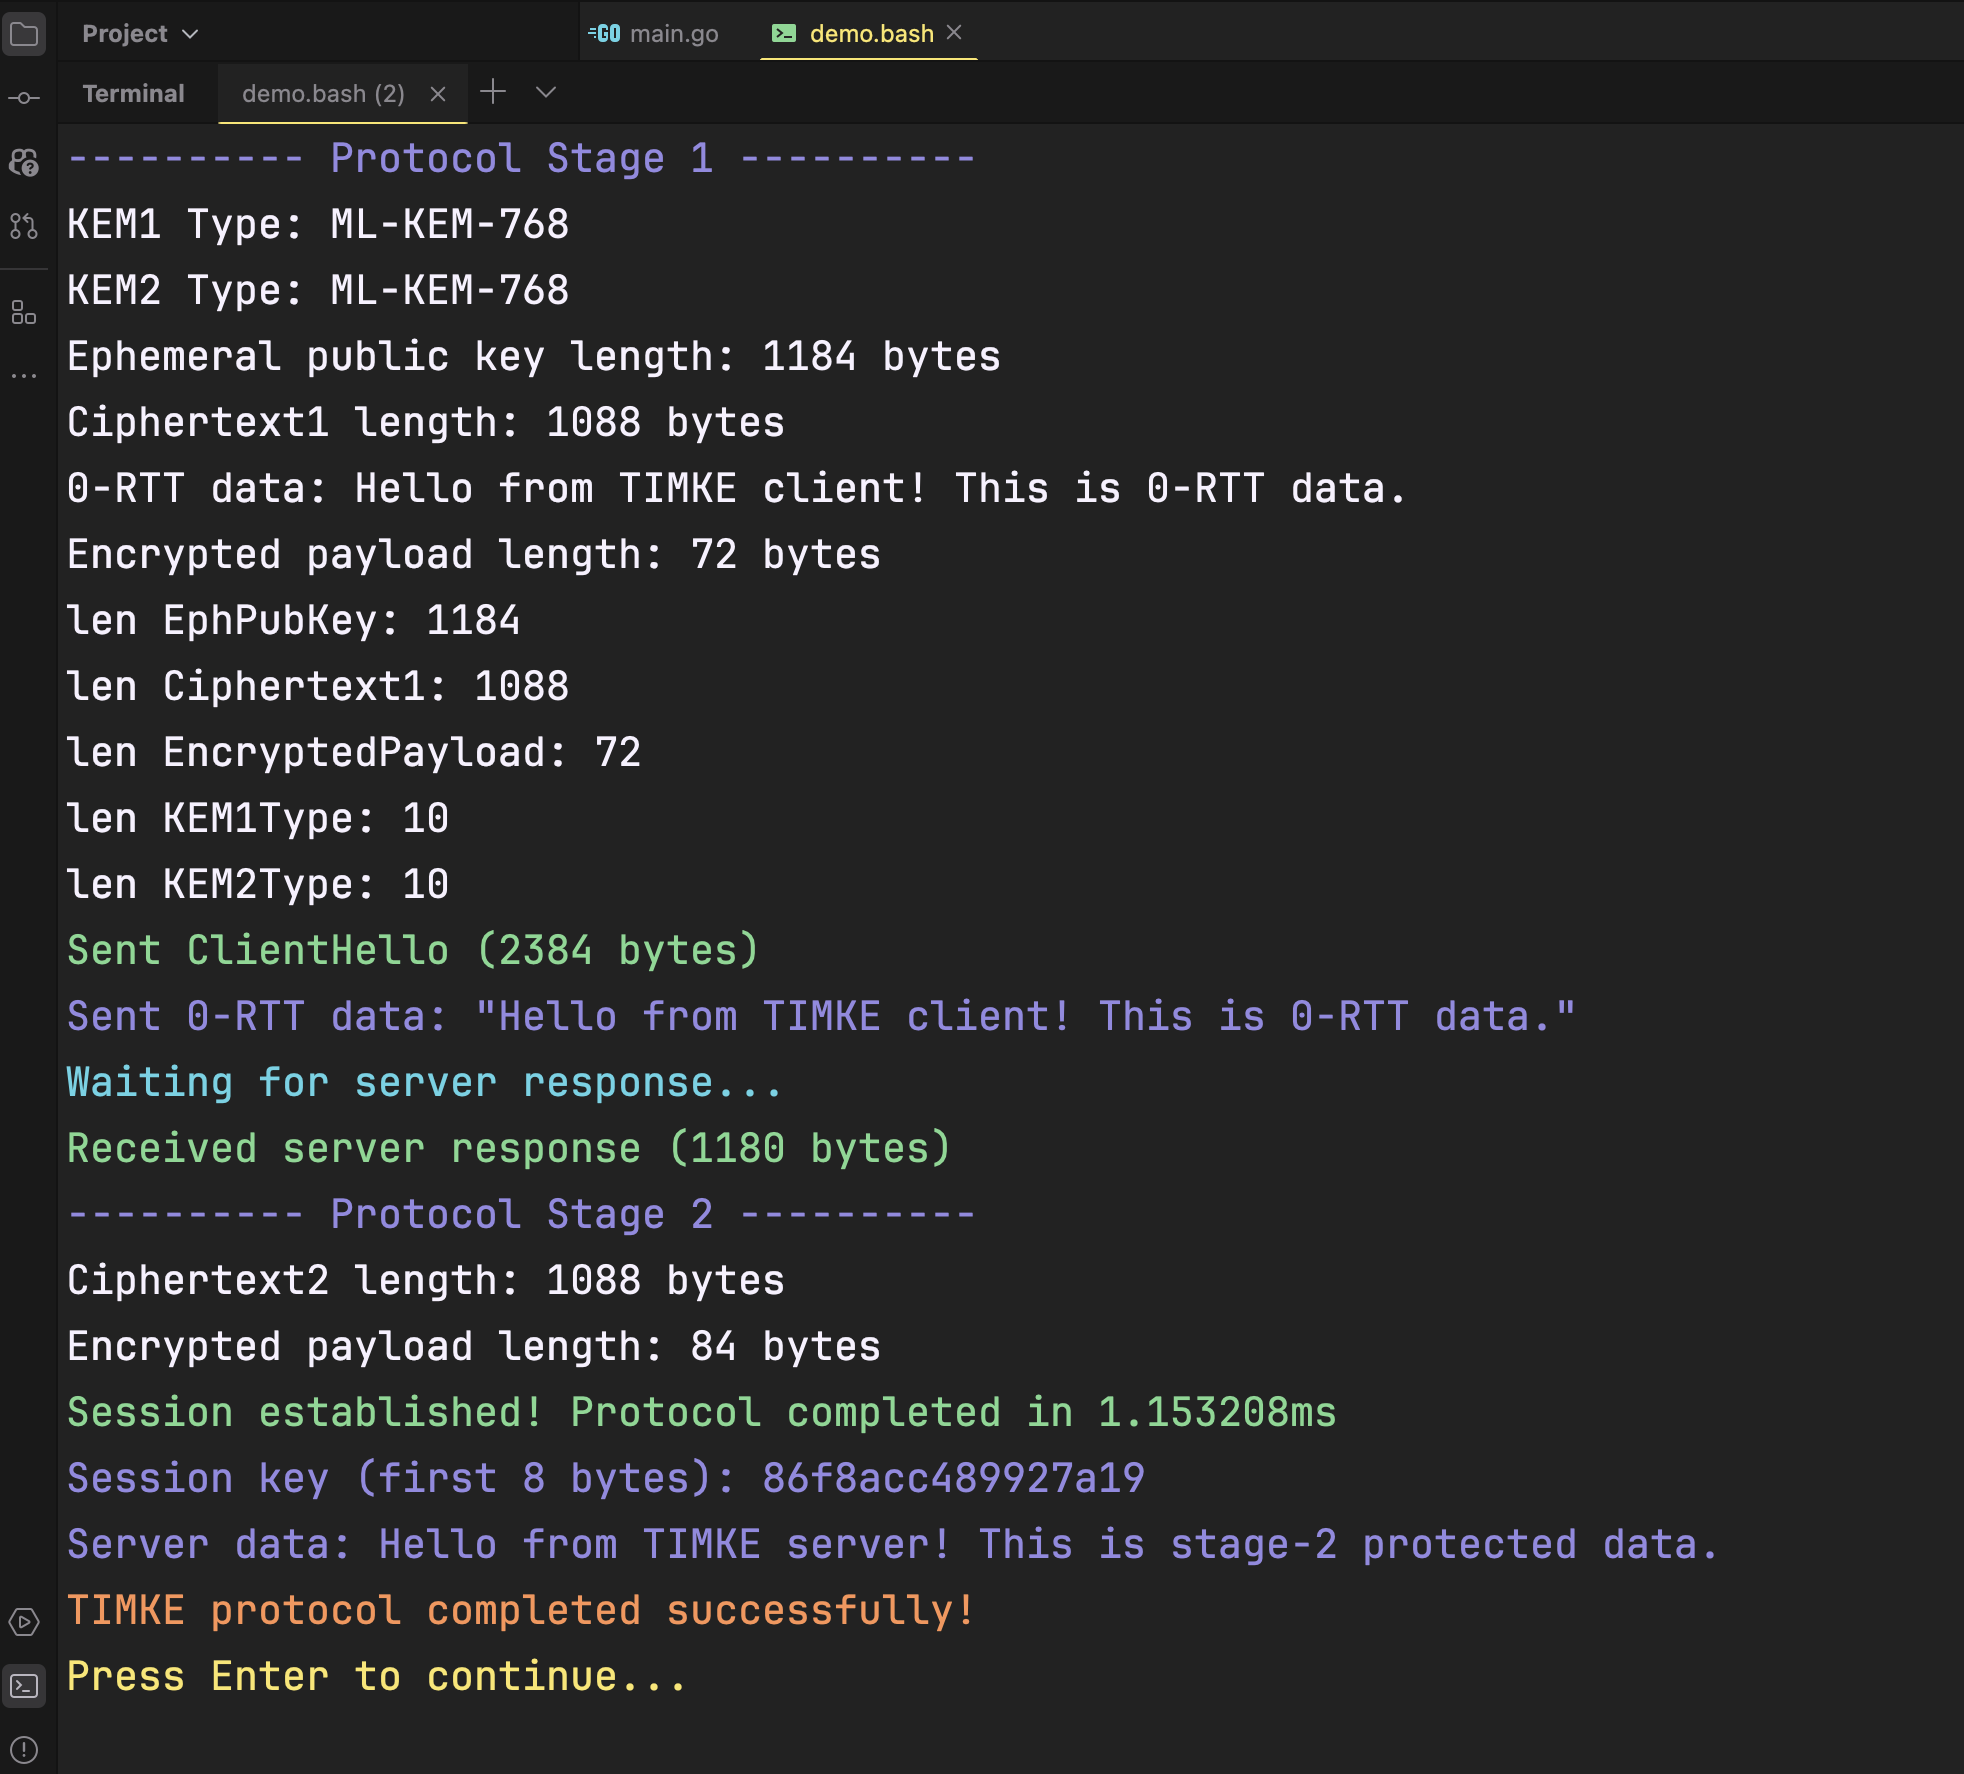
\includegraphics[width=0.9\textwidth]{figures/0rtt_demo.png}
\caption{0-RTT数据传输演示}
\label{fig:0rtt-demo}
\end{figure}

从服务器日志可以看到,服务器成功接收并解密了客户端的0-RTT数据,整个过程无需额外的往返交互,显著降低了连接建立的延迟。

\subsubsection{加密通信效果}

协议第二阶段建立的主会话密钥用于后续通信的加密保护。图\ref{fig:encrypted-comm}展示了交互式模式下的加密通信效果:

\begin{figure}[ht]
\centering
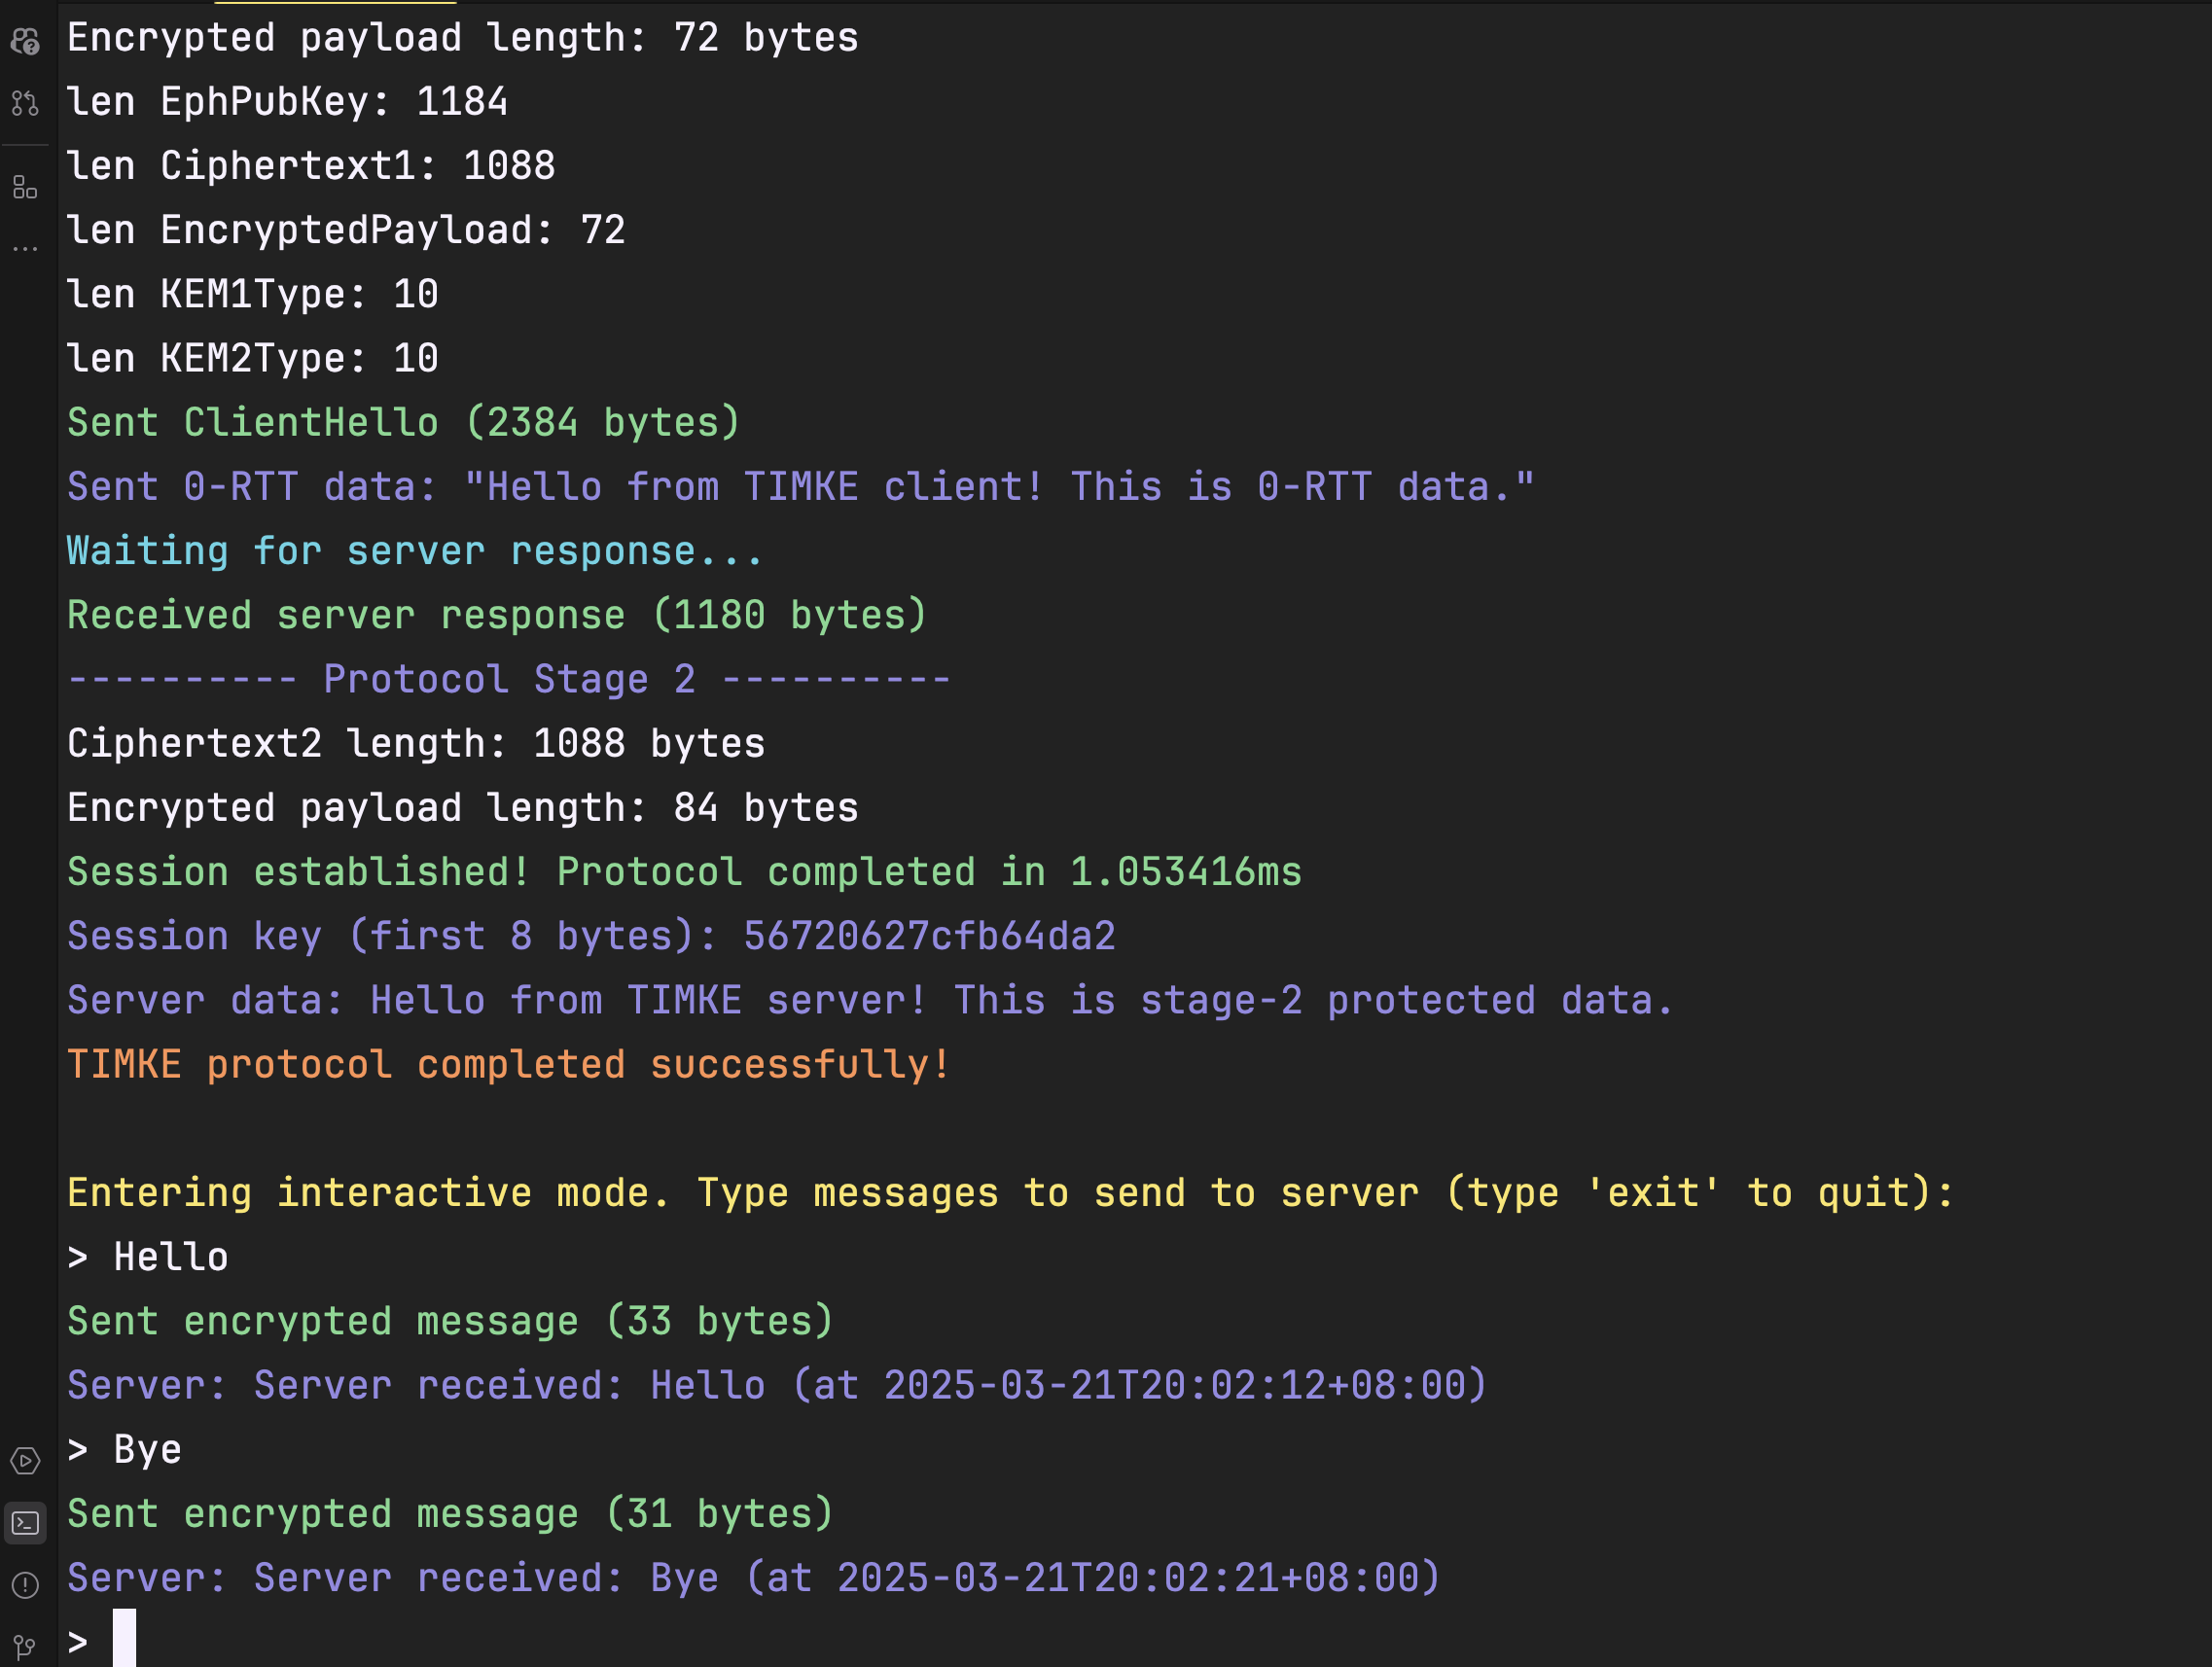
\includegraphics[width=0.9\textwidth]{figures/encrypted_comm.png}
\caption{加密通信演示}
\label{fig:encrypted-comm}
\end{figure}

所有通信内容均经过加密传输,连接双方可安全交换消息,外部观察者无法获取通信内容,实现了端到端的通信保密。

\subsubsection{内存资源使用}

不同KEM配置的内存使用情况如表\ref{tab:memory-usage}所示:

\begin{table}[ht]
\centering
\caption{不同KEM组合的内存使用情况}
\label{tab:memory-usage}
\begin{tabular}{|l|r|}
\hline
\textbf{KEM组合} & \textbf{内存使用(KB)} \\
\hline
ML-KEM-512 + ML-KEM-512    & 26   \\
\hline
ML-KEM-768 + ML-KEM-768    & 40   \\
\hline
ML-KEM-1024 + ML-KEM-1024  & 59   \\
\hline
OWChCCA-16 + ML-KEM-512    & 2,206,372   \\
\hline
\end{tabular}
\end{table}

ML-KEM配置下,协议内存占用极低,适合资源受限环境;而OWChCCA配置由于大矩阵运算需求,内存占用较高,更适合资源丰富的服务器环境。

\subsubsection{通信开销分析}

不同KEM配置的通信开销(消息大小)如表\ref{tab:comm-overhead}所示:

\begin{table}[ht]
\centering
\caption{不同KEM组合的通信开销}
\label{tab:comm-overhead}
\begin{tabular}{|l|r|r|r|}
\hline
\textbf{KEM组合} & \textbf{ClientHello(bytes)} & \textbf{ServerResponse(bytes)} & \textbf{总通信量(bytes)} \\
\hline
ML-KEM-512 + ML-KEM-512    & 1,118  & 818  & 1,936   \\
\hline
ML-KEM-768 + ML-KEM-768    & 1,438  & 1,138  & 2,576   \\
\hline
ML-KEM-1024 + ML-KEM-1024  & 1,918  & 1,618  & 3,536   \\
\hline
OWChCCA-16 + ML-KEM-512    & 8,553,228  & 818  & 8,554,046   \\
\hline
\end{tabular}
\end{table}

ML-KEM配置的通信开销控制在几KB范围内,适合各种网络环境;而OWChCCA配置由于大型公钥和密文,通信量较大,更适合高带宽环境。

综合以上演示结果,TIMKE协议在使用ML-KEM配置时展现出卓越的性能和实用性,能够在毫秒级时间内完成密钥交换,支持高效的0-RTT数据传输和安全的加密通信,同时保持低资源消耗,适合广泛的实际应用场景。
\section{开发代码}

本章将介绍TIMKE协议实现的核心代码,关注系统的关键组件和实现细节。由于篇幅限制,仅展示最具代表性的代码片段。完整代码已开源于GitHub:\url{https://github.com/MingLLuo/TIMKE/}。

\subsection{后端核心代码}

后端代码主要包括协议核心逻辑、KEM实现、消息处理和状态管理等组件。以下是几个最关键的代码片段:

\subsubsection{KEM接口定义}

KEM接口是整个系统的核心抽象,定义了密钥封装机制的标准操作集:

\begin{minted}[breaklines]{go}
// pkg/kem/interface.go
package kem

import (
    cryptoRand "crypto/rand"
    "errors"
    "io"
)

type Parameters struct {
    Name   string
    KeyLen int
}

type PublicKey interface {
    Bytes() []byte
    Algorithm() string
}

type PrivateKey interface {
    Bytes() []byte
    Algorithm() string
    PublicKey() PublicKey
}

type KEM interface {
    // 返回KEM的参数信息
    Setup() Parameters
    
    // 生成密钥对
    GenerateKeyPair(params Parameters, rand io.Reader) (PublicKey, PrivateKey, error)
    
    // 使用公钥封装共享密钥
    Encapsulate(pk PublicKey, rand io.Reader) (ciphertext []byte, sharedSecret []byte, err error)
    
    // 使用私钥解封装共享密钥
    Decapsulate(sk PrivateKey, ciphertext []byte) ([]byte, error)
    
    // 解析二进制格式的公钥
    ParsePublicKey(data []byte) (PublicKey, error)
    
    // 解析二进制格式的私钥
    ParsePrivateKey(data []byte) (PrivateKey, error)
}

var DefaultRand = cryptoRand.Reader

var (
    ErrorKEM = errors.New("kem error")
    ErrInvalidPublicKey = errors.New("invalid public key")
    ErrInvalidPrivateKey = errors.New("invalid private key")
    ErrUnsupportedKEM = errors.New("unsupported KEM type")
)
\end{minted}

该接口设计允许协议核心逻辑与具体KEM实现分离,使系统能够无缝切换不同的KEM算法。

\subsubsection{密钥派生函数实现}

密钥派生是协议安全性的关键环节,以下是H1和H2函数的实现:

\begin{minted}[breaklines]{go}
// pkg/crypto/hash.go
package crypto

import (
    "errors"
    "TIMKE/pkg/crypto/sha3"
)

type Hash struct {
    h sha3.State
}

func NewHash() *Hash {
    return &Hash{
        h: sha3.New512(),
    }
}

func (h *Hash) Hash(data ...[]byte) ([]byte, error) {
    h.h.Reset()

    for _, d := range data {
        if _, err := h.h.Write(d); err != nil {
            return nil, err
        }
    }
    return h.h.Sum(nil), nil
}

// H1 派生临时会话密钥: K_tmp = H1(pk_S, C_1, K_1)
func H1(pkS, c1, k1 []byte) ([]byte, error) {
    if pkS == nil || c1 == nil || k1 == nil {
        return nil, errors.New("invalid input to H1")
    }

    h := NewHash()
    domain := []byte("TIMKE-H1")
    return h.Hash(domain, pkS, c1, k1)
}

// H2 派生主会话密钥: K_main = H2(pk_S, epk_C, C_1, C_2, K_1, K_2)
func H2(pkS, epkC, c1, c2, k1, k2 []byte) ([]byte, error) {
    if pkS == nil || epkC == nil || c1 == nil || c2 == nil || k1 == nil || k2 == nil {
        return nil, errors.New("invalid input to H2")
    }

    h := NewHash()
    domain := []byte("TIMKE-H2")
    return h.Hash(domain, pkS, epkC, c1, c2, k1, k2)
}
\end{minted}

这些函数使用SHA3-512哈希函数,并通过域分隔标识("TIMKE-H1"和"TIMKE-H2")确保不同上下文的哈希值不会冲突。

\subsubsection{客户端实现}

客户端负责启动密钥交换流程,生成ClientHello消息并处理服务器响应:

\begin{minted}[breaklines]{go}
// pkg/protocol/client.go
package protocol

import (
    "errors"
    "fmt"
    "io"

    "TIMKE/pkg/crypto"
    "TIMKE/pkg/kem"
)

type Client struct {
    config  *Config
    state   SessionState
    options *SessionOptions
    rand    io.Reader

    ephemeralPublicKey  kem.PublicKey
    ephemeralPrivateKey kem.PrivateKey
    ciphertext1         []byte
    sharedSecret1       []byte // K_1
    tempKey             []byte // K_tmp
    ciphertext2         []byte
    sharedSecret2       []byte // K_2
    sessionKey          []byte // K_main
}

func NewClient(config *Config, options *SessionOptions) (*Client, error) {
    if config == nil {
        config = DefaultConfig()
    }

    if options == nil || options.ServerPublicKey == nil {
        return nil, errors.New("server public key is required")
    }

    return &Client{
        config:  config,
        state:   StateInitial,
        options: options,
        rand:    kem.DefaultRand,
    }, nil
}

func (c *Client) GenerateClientHello(zeroRTTData []byte) (*ClientHello, error) {
    if c.state != StateInitial {
        return nil, errors.New("client not in initial state")
    }

    // 1. 生成临时密钥对
    params := c.config.KEM2.Setup()
    epk, esk, err := c.config.KEM2.GenerateKeyPair(params, c.rand)
    if err != nil {
        c.state = StateFailed
        return nil, fmt.Errorf("failed to generate ephemeral key pair: %w", err)
    }
    c.ephemeralPublicKey = epk
    c.ephemeralPrivateKey = esk

    // 2. 使用服务器公钥封装KEM1
    c.ciphertext1, c.sharedSecret1, err = c.config.KEM1.Encapsulate(c.options.ServerPublicKey, c.rand)
    if err != nil {
        c.state = StateFailed
        return nil, fmt.Errorf("failed to encapsulate KEM1: %w", err)
    }

    // 3. 派生临时会话密钥: K_tmp = H1(server_pk, C₁, K_1)
    c.tempKey, err = crypto.H1(
        c.options.ServerPublicKey.Bytes(),
        c.ciphertext1,
        c.sharedSecret1,
    )
    if err != nil {
        c.state = StateFailed
        return nil, fmt.Errorf("failed to derive temp key: %w", err)
    }

    // 4. 加密0-RTT数据
    var encryptedPayload []byte
    if zeroRTTData != nil {
        encryptedPayload, err = c.config.SymmetricEncryption.Encrypt(c.tempKey, zeroRTTData)
        if err != nil {
            c.state = StateFailed
            return nil, fmt.Errorf("failed to encrypt 0-RTT data: %w", err)
        }
    }

    // 5. 构造ClientHello消息
    clientHello := &ClientHello{
        EphemeralPublicKey: c.ephemeralPublicKey.Bytes(),
        Ciphertext1:        c.ciphertext1,
        EncryptedPayload:   encryptedPayload,
        KEM1Type:           c.config.KEM1.Setup().Name,
        KEM2Type:           c.config.KEM2.Setup().Name,
    }

    c.state = StateAwaitingServerResponse
    return clientHello, nil
}

func (c *Client) ProcessServerResponse(response *ServerResponse) ([]byte, error) {
    if c.state != StateAwaitingServerResponse {
        return nil, errors.New("client not waiting for server response")
    }

    if response == nil {
        c.state = StateFailed
        return nil, errors.New("nil server response")
    }

    // 处理服务器响应,解封装KEM2密文
    c.ciphertext2 = response.Ciphertext2
    sharedSecret2, err := c.config.KEM2.Decapsulate(c.ephemeralPrivateKey, c.ciphertext2)
    if err != nil {
        c.state = StateFailed
        return nil, fmt.Errorf("failed to decapsulate KEM2: %w", err)
    }
    c.sharedSecret2 = sharedSecret2

    // 派生主会话密钥
    c.sessionKey, err = crypto.H2(
        c.options.ServerPublicKey.Bytes(),
        c.ephemeralPublicKey.Bytes(),
        c.ciphertext1,
        c.ciphertext2,
        c.sharedSecret1,
        c.sharedSecret2,
    )
    if err != nil {
        c.state = StateFailed
        return nil, fmt.Errorf("failed to derive session key: %w", err)
    }

    // 解密服务器有效载荷(如果有)
    var plaintext []byte
    if len(response.EncryptedPayload) > 0 {
        plaintext, err = c.config.SymmetricEncryption.Decrypt(c.sessionKey, response.EncryptedPayload)
        if err != nil {
            c.state = StateFailed
            return nil, fmt.Errorf("failed to decrypt server payload: %w", err)
        }
    }

    c.state = StateEstablished
    return plaintext, nil
}

// 其他方法...
\end{minted}

客户端实现了协议的两个阶段:生成ClientHello消息(包含临时密钥生成、KEM1封装和0-RTT数据加密)和处理服务器响应(包括KEM2解封装和主会话密钥派生)。

\subsubsection{服务器实现}

服务器负责处理客户端请求,验证身份并建立共享密钥:

\begin{minted}[breaklines]{go}
// pkg/protocol/server.go
package protocol

import (
    "errors"
    "fmt"
    "io"

    "TIMKE/pkg/crypto"
    "TIMKE/pkg/kem"
)

type Server struct {
    config  *Config
    state   SessionState
    options *SessionOptions
    rand    io.Reader

    ephemeralClientPubKey kem.PublicKey
    ciphertext1           []byte
    sharedSecret1         []byte // K_1
    tempKey               []byte // K_tmp
    ciphertext2           []byte
    sharedSecret2         []byte // K_2
    sessionKey            []byte // K_main

    dynamicKEM1 kem.KEM
    dynamicKEM2 kem.KEM
}

func NewServer(config *Config, options *SessionOptions) (*Server, error) {
    if config == nil {
        config = DefaultConfig()
    }

    if options == nil || options.ServerPrivateKey == nil {
        return nil, errors.New("server private key is required")
    }

    return &Server{
        config:  config,
        state:   StateInitial,
        options: options,
        rand:    kem.DefaultRand,
    }, nil
}

func (s *Server) ProcessClientHello(clientHello *ClientHello) ([]byte, error) {
    if s.state != StateInitial {
        return nil, errors.New("server not in initial state")
    }

    if clientHello == nil {
        s.state = StateFailed
        return nil, errors.New("nil client hello")
    }

    // 处理KEM类型协商(如果提供)
    var err error
    if clientHello.KEM1Type != "" && clientHello.KEM2Type != "" {
        s.dynamicKEM1, err = SelectKEM(clientHello.KEM1Type)
        if err != nil {
            s.dynamicKEM1 = DefaultKEM1()
        }

        s.dynamicKEM2, err = SelectKEM(clientHello.KEM2Type)
        if err != nil {
            s.dynamicKEM2 = DefaultKEM2()
        }
    } else {
        s.dynamicKEM1 = DefaultKEM1()
        s.dynamicKEM2 = DefaultKEM2()
    }

    // 1. 解析客户端临时公钥
    s.ephemeralClientPubKey, err = s.dynamicKEM2.ParsePublicKey(clientHello.EphemeralPublicKey)
    if err != nil {
        s.state = StateFailed
        return nil, fmt.Errorf("failed to parse ephemeral public key: %w", err)
    }

    s.ciphertext1 = clientHello.Ciphertext1

    // 2. 使用服务器私钥解封装KEM1密文
    s.sharedSecret1, err = s.dynamicKEM1.Decapsulate(s.options.ServerPrivateKey, s.ciphertext1)
    if err != nil {
        s.state = StateFailed
        return nil, fmt.Errorf("failed to decapsulate KEM1: %w", err)
    }

    // 3. 派生临时会话密钥
    serverPubKey := s.options.ServerPrivateKey.PublicKey()
    s.tempKey, err = crypto.H1(
        serverPubKey.Bytes(),
        s.ciphertext1,
        s.sharedSecret1,
    )
    if err != nil {
        s.state = StateFailed
        return nil, fmt.Errorf("failed to derive temp key: %w", err)
    }

    // 4. 解密0-RTT数据(如果有)
    var zeroRTTData []byte
    if len(clientHello.EncryptedPayload) > 0 {
        zeroRTTData, err = s.config.SymmetricEncryption.Decrypt(s.tempKey, clientHello.EncryptedPayload)
        if err != nil {
            s.state = StateFailed
            return nil, fmt.Errorf("failed to decrypt 0-RTT data: %w", err)
        }
    }

    return zeroRTTData, nil
}

func (s *Server) GenerateServerResponse(payload []byte) (*ServerResponse, error) {
    if s.ephemeralClientPubKey == nil || s.sharedSecret1 == nil {
        return nil, errors.New("client hello not processed")
    }

    // 1. 使用客户端临时公钥封装KEM2
    var err error
    s.ciphertext2, s.sharedSecret2, err = s.dynamicKEM2.Encapsulate(s.ephemeralClientPubKey, s.rand)
    if err != nil {
        s.state = StateFailed
        return nil, fmt.Errorf("failed to encapsulate KEM2: %w", err)
    }

    // 2. 派生主会话密钥
    serverPubKey := s.options.ServerPrivateKey.PublicKey()
    s.sessionKey, err = crypto.H2(
        serverPubKey.Bytes(),
        s.ephemeralClientPubKey.Bytes(),
        s.ciphertext1,
        s.ciphertext2,
        s.sharedSecret1,
        s.sharedSecret2,
    )
    if err != nil {
        s.state = StateFailed
        return nil, fmt.Errorf("failed to derive session key: %w", err)
    }

    // 3. 加密有效载荷(如果有)
    var encryptedPayload []byte
    if payload != nil {
        encryptedPayload, err = s.config.SymmetricEncryption.Encrypt(s.sessionKey, payload)
        if err != nil {
            s.state = StateFailed
            return nil, fmt.Errorf("failed to encrypt payload: %w", err)
        }
    }

    // 4. 构造服务器响应
    serverResponse := &ServerResponse{
        Ciphertext2:      s.ciphertext2,
        EncryptedPayload: encryptedPayload,
    }

    s.state = StateEstablished
    return serverResponse, nil
}

// 其他方法...
\end{minted}

服务器实现了协议的两个主要功能:处理ClientHello消息(包括解析临时公钥、解封装KEM1密文和解密0-RTT数据)和生成ServerResponse(包括KEM2封装和有效载荷加密)。

\subsubsection{消息序列化}

协议消息的序列化是确保通信正确性的关键组件:

\begin{minted}[breaklines]{go}
// pkg/protocol/serializer.go
package protocol

import (
    "encoding/binary"
    "errors"
    "fmt"
)

// 消息结构定义
type ClientHello struct {
    EphemeralPublicKey []byte
    Ciphertext1        []byte
    EncryptedPayload   []byte
    KEM1Type           string
    KEM2Type           string
}

type ServerResponse struct {
    Ciphertext2      []byte
    EncryptedPayload []byte
}

// DefaultSerializer 实现消息序列化接口
type DefaultSerializer struct{}

// MarshalClientHello 序列化ClientHello消息
func (s *DefaultSerializer) MarshalClientHello(ch *ClientHello) ([]byte, error) {
    if ch == nil {
        return nil, errors.New("cannot marshal nil ClientHello")
    }

    // 预分配合理大小的缓冲区
    estimatedSize := 4 + len(ch.EphemeralPublicKey) +
        4 + len(ch.Ciphertext1) +
        4 + len(ch.EncryptedPayload) +
        4 + len([]byte(ch.KEM1Type)) +
        4 + len([]byte(ch.KEM2Type))

    result := make([]byte, 0, estimatedSize)

    // 使用长度前缀编码每个字段
    result = writeLengthPrefixedBytes(result, ch.EphemeralPublicKey)
    result = writeLengthPrefixedBytes(result, ch.Ciphertext1)
    result = writeLengthPrefixedBytes(result, ch.EncryptedPayload)
    result = writeLengthPrefixedBytes(result, []byte(ch.KEM1Type))
    result = writeLengthPrefixedBytes(result, []byte(ch.KEM2Type))

    return result, nil
}

// UnmarshalClientHello 反序列化ClientHello消息
func (s *DefaultSerializer) UnmarshalClientHello(data []byte) (*ClientHello, error) {
    if len(data) < 2 {
        return nil, ErrInvalidMessage
    }

    ch := &ClientHello{}
    offset := 0
    var err error

    // 读取各字段
    ch.EphemeralPublicKey, offset, err = readLengthPrefixedBytes(data, offset)
    if err != nil {
        return nil, err
    }

    ch.Ciphertext1, offset, err = readLengthPrefixedBytes(data, offset)
    if err != nil {
        return nil, err
    }

    ch.EncryptedPayload, offset, err = readLengthPrefixedBytes(data, offset)
    if err != nil {
        return nil, err
    }

    kem1TypeBytes, offset, err := readLengthPrefixedBytes(data, offset)
    if err != nil {
        return nil, err
    }
    ch.KEM1Type = string(kem1TypeBytes)

    kem2TypeBytes, offset, err := readLengthPrefixedBytes(data, offset)
    if err != nil {
        return nil, err
    }
    ch.KEM2Type = string(kem2TypeBytes)

    // 检查是否已读取全部数据
    if offset != len(data) {
        return ch, errors.New("extra data after message")
    }

    return ch, nil
}

// 辅助函数
func readLengthPrefixedBytes(data []byte, offset int) ([]byte, int, error) {
    // 检查是否可以读取长度字段(4字节)
    if offset+4 > len(data) {
        return nil, offset, ErrBufferTooShort
    }

    // 读取长度
    length := binary.BigEndian.Uint32(data[offset:])
    offset += 4

    // 检查是否可以读取数据
    if offset+int(length) > len(data) {
        return nil, offset, ErrBufferTooShort
    }

    // 提取数据
    result := make([]byte, length)
    copy(result, data[offset:offset+int(length)])
    offset += int(length)

    return result, offset, nil
}

func writeLengthPrefixedBytes(result []byte, data []byte) []byte {
    // 分配4字节存储长度
    lengthBytes := make([]byte, 4)
    binary.BigEndian.PutUint32(lengthBytes, uint32(len(data)))

    // 追加长度和数据
    result = append(result, lengthBytes...)
    result = append(result, data...)

    return result
}

// 其他序列化方法...
\end{minted}
消息序列化代码定义了ClientHello和ServerResponse消息的格式,并提供了序列化和反序列化方法,使用长度前缀编码确保消息的正确解析。

\subsection{前端核心代码}

TIMKE协议实现主要为命令行应用,包含客户端和服务器两个前端程序,以及演示脚本。

\subsubsection{客户端程序}

客户端程序提供命令行接口,支持与服务器建立TIMKE会话:

\begin{minted}[breaklines]{go}
// cmd/client/main.go
package main

import (
    "bufio"
    "encoding/binary"
    "encoding/hex"
    "flag"
    "fmt"
    "io"
    "log"
    "net"
    "os"
    "strings"
    "time"

    "TIMKE/pkg/kem"
    "TIMKE/pkg/protocol"
)

// 颜色常量定义
const (
    colorReset  = "\033[0m"
    colorRed    = "\033[31m"
    colorGreen  = "\033[32m"
    colorYellow = "\033[33m"
    colorBlue   = "\033[34m"
    colorPurple = "\033[35m"
    colorCyan   = "\033[36m"
)

func main() {
    // 命令行参数定义
    var (
        host          = flag.String("host", "localhost", "服务器主机名或IP")
        port          = flag.Int("port", 8443, "服务器端口")
        serverPubKey  = flag.String("server-key", "", "服务器公钥(十六进制格式)")
        serverKeyFile = flag.String("server-key-file", "", "包含服务器公钥的文件路径")
        kem1Type      = flag.String("kem1", "ML-KEM-768", "服务器密钥KEM类型")
        kem2Type      = flag.String("kem2", "ML-KEM-768", "临时密钥KEM类型")
        zeroRTTMsg    = flag.String("0rtt", "Hello from TIMKE client! This is 0-RTT data.", "0-RTT消息(空字符串禁用)")
        interactive   = flag.Bool("i", false, "交互模式(密钥交换后发送/接收消息)")
        verbose       = flag.Bool("v", false, "显示详细输出")
    )
    flag.Parse()

    logger := log.New(os.Stdout, "", 0)

    // 打印标题
    printBanner(logger)

    // 列出可用的KEM算法
    logger.Printf("%s可用的KEM算法:%s\n", colorYellow, colorReset)
    for _, k := range kem.ListKEMs() {
        logger.Printf("  - %s\n", k)
    }
    logger.Println()

    // 获取服务器公钥
    var serverPublicKeyBytes []byte
    var err error

    if *serverKeyFile != "" {
        // 从文件加载
        serverPublicKeyBytes, err = os.ReadFile(*serverKeyFile)
        if err != nil {
            logger.Fatalf("%s读取服务器密钥文件错误: %s%s\n", colorRed, err, colorReset)
        }
    } else if *serverPubKey != "" {
        // 解析十六进制字符串
        serverPublicKeyBytes, err = hex.DecodeString(*serverPubKey)
        if err != nil {
            logger.Fatalf("%s解码服务器公钥错误: %s%s\n", colorRed, err, colorReset)
        }
    } else {
        logger.Fatalf("%s错误: 必须提供--server-key或--server-key-file参数%s\n", colorRed, colorReset)
    }

    // 获取KEM实例
    kem1, err := kem.GetKEM(*kem1Type)
    if err != nil {
        logger.Fatalf("%s错误: KEM1类型'%s'未找到: %s%s\n", colorRed, *kem1Type, err, colorReset)
    }
    kem2, err := kem.GetKEM(*kem2Type)
    if err != nil {
        logger.Fatalf("%s错误: KEM2类型'%s'未找到: %s%s\n", colorRed, *kem2Type, err, colorReset)
    }

    // 解析服务器公钥
    serverPublicKey, err := kem1.ParsePublicKey(serverPublicKeyBytes)
    if err != nil {
        logger.Fatalf("%s解析服务器公钥错误: %s%s\n", colorRed, err, colorReset)
    }

    logger.Printf("%s使用服务器密钥: %s%s\n", colorGreen, serverPublicKey.Algorithm(), colorReset)

    // 创建客户端配置
    config := &protocol.Config{
        KEM1:                kem1,
        KEM2:                kem2,
        SymmetricEncryption: protocol.DefaultConfig().SymmetricEncryption,
    }

    // 创建客户端选项
    options := protocol.NewSessionOptions().WithServerPublicKey(serverPublicKey)

    // 创建客户端
    client, err := protocol.NewClient(config, options)
    if err != nil {
        logger.Fatalf("%s创建客户端错误: %s%s\n", colorRed, err, colorReset)
    }

    // 连接服务器
    serverAddr := fmt.Sprintf("%s:%d", *host, *port)
    logger.Printf("%s连接到%s...%s\n", colorYellow, serverAddr, colorReset)
    conn, err := net.Dial("tcp", serverAddr)
    if err != nil {
        logger.Fatalf("%s连接服务器错误: %s%s\n", colorRed, err, colorReset)
    }
    defer conn.Close()
    logger.Printf("%s已连接到%s%s\n", colorGreen, serverAddr, colorReset)

    // 准备0-RTT数据
    var zeroRTTData []byte
    if *zeroRTTMsg != "" {
        zeroRTTData = []byte(*zeroRTTMsg)
    }

    // 开始协议 - 生成ClientHello
    startTime := time.Now()
    logger.Printf("%s生成ClientHello...%s\n", colorCyan, colorReset)
    clientHello, err := client.GenerateClientHello(zeroRTTData)
    if err != nil {
        logger.Fatalf("%s生成ClientHello错误: %s%s\n", colorRed, err, colorReset)
    }

    // 协议可视化 - 第一阶段
    if *verbose {
        logger.Printf("%s---------- 协议第一阶段 ----------%s\n", colorPurple, colorReset)
        logger.Printf("KEM1类型: %s\n", clientHello.KEM1Type)
        logger.Printf("KEM2类型: %s\n", clientHello.KEM2Type)
        logger.Printf("临时公钥长度: %d字节\n", len(clientHello.EphemeralPublicKey))
        logger.Printf("密文1长度: %d字节\n", len(clientHello.Ciphertext1))
        if zeroRTTData != nil {
            logger.Printf("0-RTT数据: %s\n", *zeroRTTMsg)
            logger.Printf("加密载荷长度: %d字节\n", len(clientHello.EncryptedPayload))
        } else {
            logger.Printf("无0-RTT数据\n")
        }
    }

    // 序列化并发送ClientHello
    serializer := &protocol.DefaultSerializer{}
    clientHelloBytes, err := serializer.MarshalClientHello(clientHello)
    if err != nil {
        logger.Fatalf("%s序列化ClientHello错误: %s%s\n", colorRed, err, colorReset)
    }

    // 首先发送长度(4字节,32位)
    lenBuf := make([]byte, 4)
    binary.BigEndian.PutUint32(lenBuf, uint32(len(clientHelloBytes)))
    if _, err := conn.Write(lenBuf); err != nil {
        logger.Fatalf("%s发送ClientHello长度错误: %s%s\n", colorRed, err, colorReset)
    }

    // 然后发送实际的ClientHello
    if _, err := conn.Write(clientHelloBytes); err != nil {
        logger.Fatalf("%s发送ClientHello错误: %s%s\n", colorRed, err, colorReset)
    }

    logger.Printf("%s已发送ClientHello (%d字节)%s\n", colorGreen, len(clientHelloBytes), colorReset)
    if zeroRTTData != nil {
        logger.Printf("%s已发送0-RTT数据: \"%s\"%s\n", colorPurple, *zeroRTTMsg, colorReset)
    }

    // 读取服务器响应
    logger.Printf("%s等待服务器响应...%s\n", colorCyan, colorReset)

    // 读取消息长度
    if _, err := io.ReadFull(conn, lenBuf); err != nil {
        logger.Fatalf("%s读取服务器响应长度错误: %s%s\n", colorRed, err, colorReset)
    }

    messageLen := int(binary.BigEndian.Uint32(lenBuf))
    messageBuf := make([]byte, messageLen)
    if _, err := io.ReadFull(conn, messageBuf); err != nil {
        logger.Fatalf("%s读取服务器响应错误: %s%s\n", colorRed, err, colorReset)
    }

    // 反序列化服务器响应
    serverResponse, err := serializer.UnmarshalServerResponse(messageBuf)
    if err != nil {
        logger.Fatalf("%s反序列化服务器响应错误: %s%s\n", colorRed, err, colorReset)
    }

    logger.Printf("%s收到服务器响应 (%d字节)%s\n", colorGreen, len(messageBuf), colorReset)

    // 协议可视化 - 第二阶段
    if *verbose {
        logger.Printf("%s---------- 协议第二阶段 ----------%s\n", colorPurple, colorReset)
        logger.Printf("密文2长度: %d字节\n", len(serverResponse.Ciphertext2))
        logger.Printf("加密载荷长度: %d字节\n", len(serverResponse.EncryptedPayload))
    }

    // 处理服务器响应
    serverData, err := client.ProcessServerResponse(serverResponse)
    if err != nil {
        logger.Fatalf("%s处理服务器响应错误: %s%s\n", colorRed, err, colorReset)
    }

    elapsedTime := time.Since(startTime)
    sessionKey := client.GetSessionKey()

    // 会话已建立!
    logger.Printf("%s会话已建立! 协议完成时间: %v%s\n", colorGreen, elapsedTime, colorReset)
    if *verbose && len(sessionKey) > 0 {
        logger.Printf("%s会话密钥(前8字节): %x%s\n", colorPurple, sessionKey[:min(8, len(sessionKey))], colorReset)
    }

    // 显示服务器数据
    if len(serverData) > 0 {
        logger.Printf("%s服务器数据: %s%s\n", colorPurple, string(serverData), colorReset)
    }

    // 协议完成!
    logger.Printf("%sTIMKE协议成功完成!%s\n", colorBlue, colorReset)

    // 交互模式
    if *interactive {
        // 实现交互式消息收发...
    }
}

// 其他辅助函数...
\end{minted}

客户端程序提供了用户友好的命令行接口,支持多种参数配置,并通过颜色编码输出增强用户体验。程序实现了完整的TIMKE协议交互流程,包括建立连接、发送ClientHello、处理服务器响应和显示会话状态。

\subsubsection{演示脚本}

演示脚本提供了用户友好的交互式界面,整合了协议的所有功能:

\begin{minted}[breaklines]{bash}
#!/bin/bash

# 颜色定义
RED='\033[0;31m'
GREEN='\033[0;32m'
YELLOW='\033[0;33m'
BLUE='\033[0;34m'
CYAN='\033[0;36m'
NC='\033[0m' # No Color

# 默认设置
KEM1_TYPE="ML-KEM-768"
KEM2_TYPE="ML-KEM-768"
PORT=8443
TEMP_DIR="$(pwd)/.temp"
SERVER_KEY="${TEMP_DIR}/server-key.pem"
CLIENT_ZERO_RTT="Hello from TIMKE client! This is 0-RTT data."
SERVER_PID_FILE="${TEMP_DIR}/server.pid"

# 标题
...

# 解析命令行参数
while [[ $# -gt 0 ]]; do
    case $1 in
        --kem1)
            KEM1_TYPE="$2"
            shift 2
            ;;
        --kem2)
            KEM2_TYPE="$2"
            shift 2
            ;;
        --port)
            PORT="$2"
            shift 2
            ;;
        --help)
            print_banner
            echo -e "${GREEN}TIMKE演示运行脚本${NC}"
            echo -e "用法: $0 [选项]"
            echo -e ""
            echo -e "选项:"
            echo -e "  --kem1 TYPE     要使用的KEM1算法 (默认: ML-KEM-768)"
            echo -e "  --kem2 TYPE     要使用的KEM2算法 (默认: ML-KEM-768)"
            echo -e "  --port PORT     服务器端口 (默认: 8443)"
            echo -e "  --help          显示帮助信息"
            exit 0
            ;;
        *)
            echo -e "${RED}未知选项: $1${NC}"
            exit 1
            ;;
    esac
done

# 退出时清理
cleanup() {
    echo -e "${YELLOW}清理临时文件...${NC}"
    
    # 检查服务器是否运行,如果是则停止
    if [ -f "${SERVER_PID_FILE}" ]; then
        SERVER_PID=$(cat "${SERVER_PID_FILE}")
        if kill -0 "${SERVER_PID}" 2>/dev/null; then
            echo -e "${YELLOW}停止TIMKE服务器 (PID: ${SERVER_PID})...${NC}"
            kill "${SERVER_PID}" 2>/dev/null || true
        fi
    fi
}

# 生成服务器密钥
generate_keys() {
    echo -e "${YELLOW}使用kem1.(${KEM1_TYPE})生成服务器密钥...${NC}"

    # 移动到项目根目录
    cd "$(dirname "$0")/.." || exit 1
    # 检查临时目录是否存在
    if [[ ! -d "${TEMP_DIR}" ]]; then
        mkdir -p "${TEMP_DIR}"
    fi

    go run ./cmd/server/main.go --genkey "${SERVER_KEY}" --kem1 "${KEM1_TYPE}" --kem2 "${KEM2_TYPE}"
    
    if [[ ! -f "${SERVER_KEY}" || ! -f "${SERVER_KEY}.pub" ]]; then
        echo -e "${RED}生成服务器密钥失败.${NC}"
        return 1
    fi
    
    echo -e "${GREEN}服务器密钥已生成:${NC}"
    echo -e "  私钥: ${SERVER_KEY}"
    echo -e "  公钥: ${SERVER_KEY}.pub"
    echo -e "\n"
    
    return 0
}

# 启动服务器
start_server() {
    # 移动到项目根目录
    cd "$(dirname "$0")/.." || exit 1

    # 检查临时目录是否存在
    if [[ ! -d "${TEMP_DIR}" ]]; then
        mkdir -p "${TEMP_DIR}"
    fi

    # 检查服务器是否已经运行
    if [ -f "${SERVER_PID_FILE}" ]; then
        local old_pid=$(cat "${SERVER_PID_FILE}")
        if kill -0 "${old_pid}" 2>/dev/null; then
            echo -e "${YELLOW}服务器已在运行中,PID: ${old_pid}${NC}"
            return 0
        fi
    fi

    # 检查密钥是否存在
    if [[ ! -f "${SERVER_KEY}" ]]; then
        echo -e "${RED}未找到服务器密钥。请先生成密钥.${NC}"
        return 1
    fi

    echo -e "${YELLOW}在端口 ${PORT} 上启动TIMKE服务器...${NC}"
    
    # 后台启动服务器
    TIMESTAMP=$(date +"%Y-%m-%d_%H-%M-%S")
    echo "TIMKE服务器日志文件" > "${TEMP_DIR}/server.log"
    echo "时间戳: ${TIMESTAMP}" >> "${TEMP_DIR}/server.log"
    go run ./cmd/server/main.go --key "${SERVER_KEY}" --port "${PORT}" --kem1 "${KEM1_TYPE}" --kem2 "${KEM2_TYPE}" --v > "${TEMP_DIR}/server.log" 2>&1 &
    local server_pid=$!
    
    # 保存PID用于后续清理
    echo "${server_pid}" > "${SERVER_PID_FILE}"
    
    # 等待片刻让服务器启动
    sleep 2
    
    # 检查服务器是否运行
    if ! kill -0 "${server_pid}" 2>/dev/null; then
        echo -e "${RED}服务器启动失败。查看服务器日志: ${TEMP_DIR}/server.log${NC}"
        cat "${TEMP_DIR}/server.log"
        return 1
    fi
    
    echo -e "${GREEN}服务器已启动,PID: ${server_pid}${NC}"
    echo -e "${BLUE}服务器日志路径: ${TEMP_DIR}/server.log${NC}"
    echo -e "${YELLOW}服务器日志尾部:${NC}"
    tail -n 10 "${TEMP_DIR}/server.log"
    echo
    
    return 0
}

# 其他功能实现...

# 注册清理函数
trap cleanup EXIT

# 主菜单
show_menu() {
    echo -e "${GREEN}TIMKE演示选项:${NC}"
    echo -e "  ${YELLOW}1)${NC} 生成服务器密钥"
    echo -e "  ${YELLOW}2)${NC} 启动服务器"
    echo -e "  ${YELLOW}3)${NC} 运行携带0-RTT数据的客户端"
    echo -e "  ${YELLOW}4)${NC} 运行交互式客户端"
    echo -e "  ${YELLOW}5)${NC} 显示服务器日志"
    echo -e "  ${YELLOW}6)${NC} 停止服务器"
    echo -e "  ${YELLOW}7)${NC} 退出"
    echo
    echo -e "${BLUE}使用KEM1: ${KEM1_TYPE}, KEM2: ${KEM2_TYPE}, 端口: ${PORT}${NC}"
    echo
    
    # 检查服务器状态
    if [ -f "${SERVER_PID_FILE}" ]; then
        local pid=$(cat "${SERVER_PID_FILE}")
        if kill -0 "${pid}" 2>/dev/null; then
            echo -e "${GREEN}服务器正在运行,PID: ${pid}${NC}"
        else
            echo -e "${RED}服务器未运行(过期的PID文件)${NC}"
            rm -f "${SERVER_PID_FILE}"
        fi
    else
        echo -e "${YELLOW}服务器未运行${NC}"
    fi
    echo
}

# 主循环
print_banner

while true; do
    show_menu
    echo -n "输入您的选择 [1-7]: "
    read -r choice
    
    case $choice in
        1)
            generate_keys
            echo -e "${YELLOW}按Enter继续...${NC}"
            read -r
            ;;
        2)
            start_server
            echo -e "${YELLOW}按Enter继续...${NC}"
            read -r
            ;;
        3)
            run_client_0rtt
            echo -e "${YELLOW}按Enter继续...${NC}"
            read -r
            ;;
        4)
            run_client_interactive
            ;;
        5)
            show_server_log
            echo -e "${YELLOW}按Enter继续...${NC}"
            read -r
            ;;
        6)
            stop_server
            echo -e "${YELLOW}按Enter继续...${NC}"
            read -r
            ;;
        7)
            echo -e "${GREEN}退出TIMKE演示.${NC}"
            exit 0
            ;;
        *)
            echo -e "${RED}无效选择。请输入1到7之间的数字.${NC}"
            sleep 1
            ;;
    esac
    
    clear
    print_banner
done
\end{minted}

演示脚本提供了用户友好的菜单界面,集成了服务器密钥生成、服务器启动、客户端连接等所有核心功能,使用户能够轻松体验TIMKE协议的完整流程,是展示系统功能的重要工具。

通过以上代码示例,展示了TIMKE协议实现的核心组件和关键逻辑。完整代码实现了更多功能和优化,可在GitHub代码库中查看。
\end{spacing}

% 结束计算页码
\setboolean{@twoside}{false}

\end{document}